\documentclass{article}

% these packages let you do math
\usepackage{amsmath}
\usepackage{amssymb}

% we need these packages for fancy R tables
\usepackage{booktabs}
\usepackage{float}
\usepackage{colortbl}
\usepackage{xcolor}

% these packages play with the spacing/margins of the document. Uncomment the commands on lines 16 and 17 to see what they do.
\usepackage{a4wide}
\usepackage{setspace}
\usepackage{geometry}
\usepackage{parskip}
%\doublespacing
%\geometry{margin=1.5in}

% this package helps us with including images. Setting the graphics path makes it easier to refer to things in the \includegraphics command.
\usepackage{graphicx}
\graphicspath{ {../figures/} }

% make some hyperlinks using the \href command
\usepackage{hyperref}
\hypersetup{
    colorlinks=true,
    linkcolor=black,
    urlcolor=blue
}

% set the author, title, and date of the document. \maketitle adds it to the document.
\author{John Walkington}
\title{Hidden Curriculum Assignment: NLSY97 Data}
\date{Spring 2022}

\begin{document}
\maketitle

\section{Analysis}

On average, black men spent the most time in jail in 2002.  Perhaps this could be because black men on average are sentenced more harshly.  It could also be that black men typically commit crimes that carry more severe sentences.  There is a significant increase in average incarceration length for all men, and a significant decrease in average incarceration length for whites.  There is not analysis to happen to determine if this is bias or a latent correlation with something unobserved.

\begin{figure}[H]
    \begin{center}
        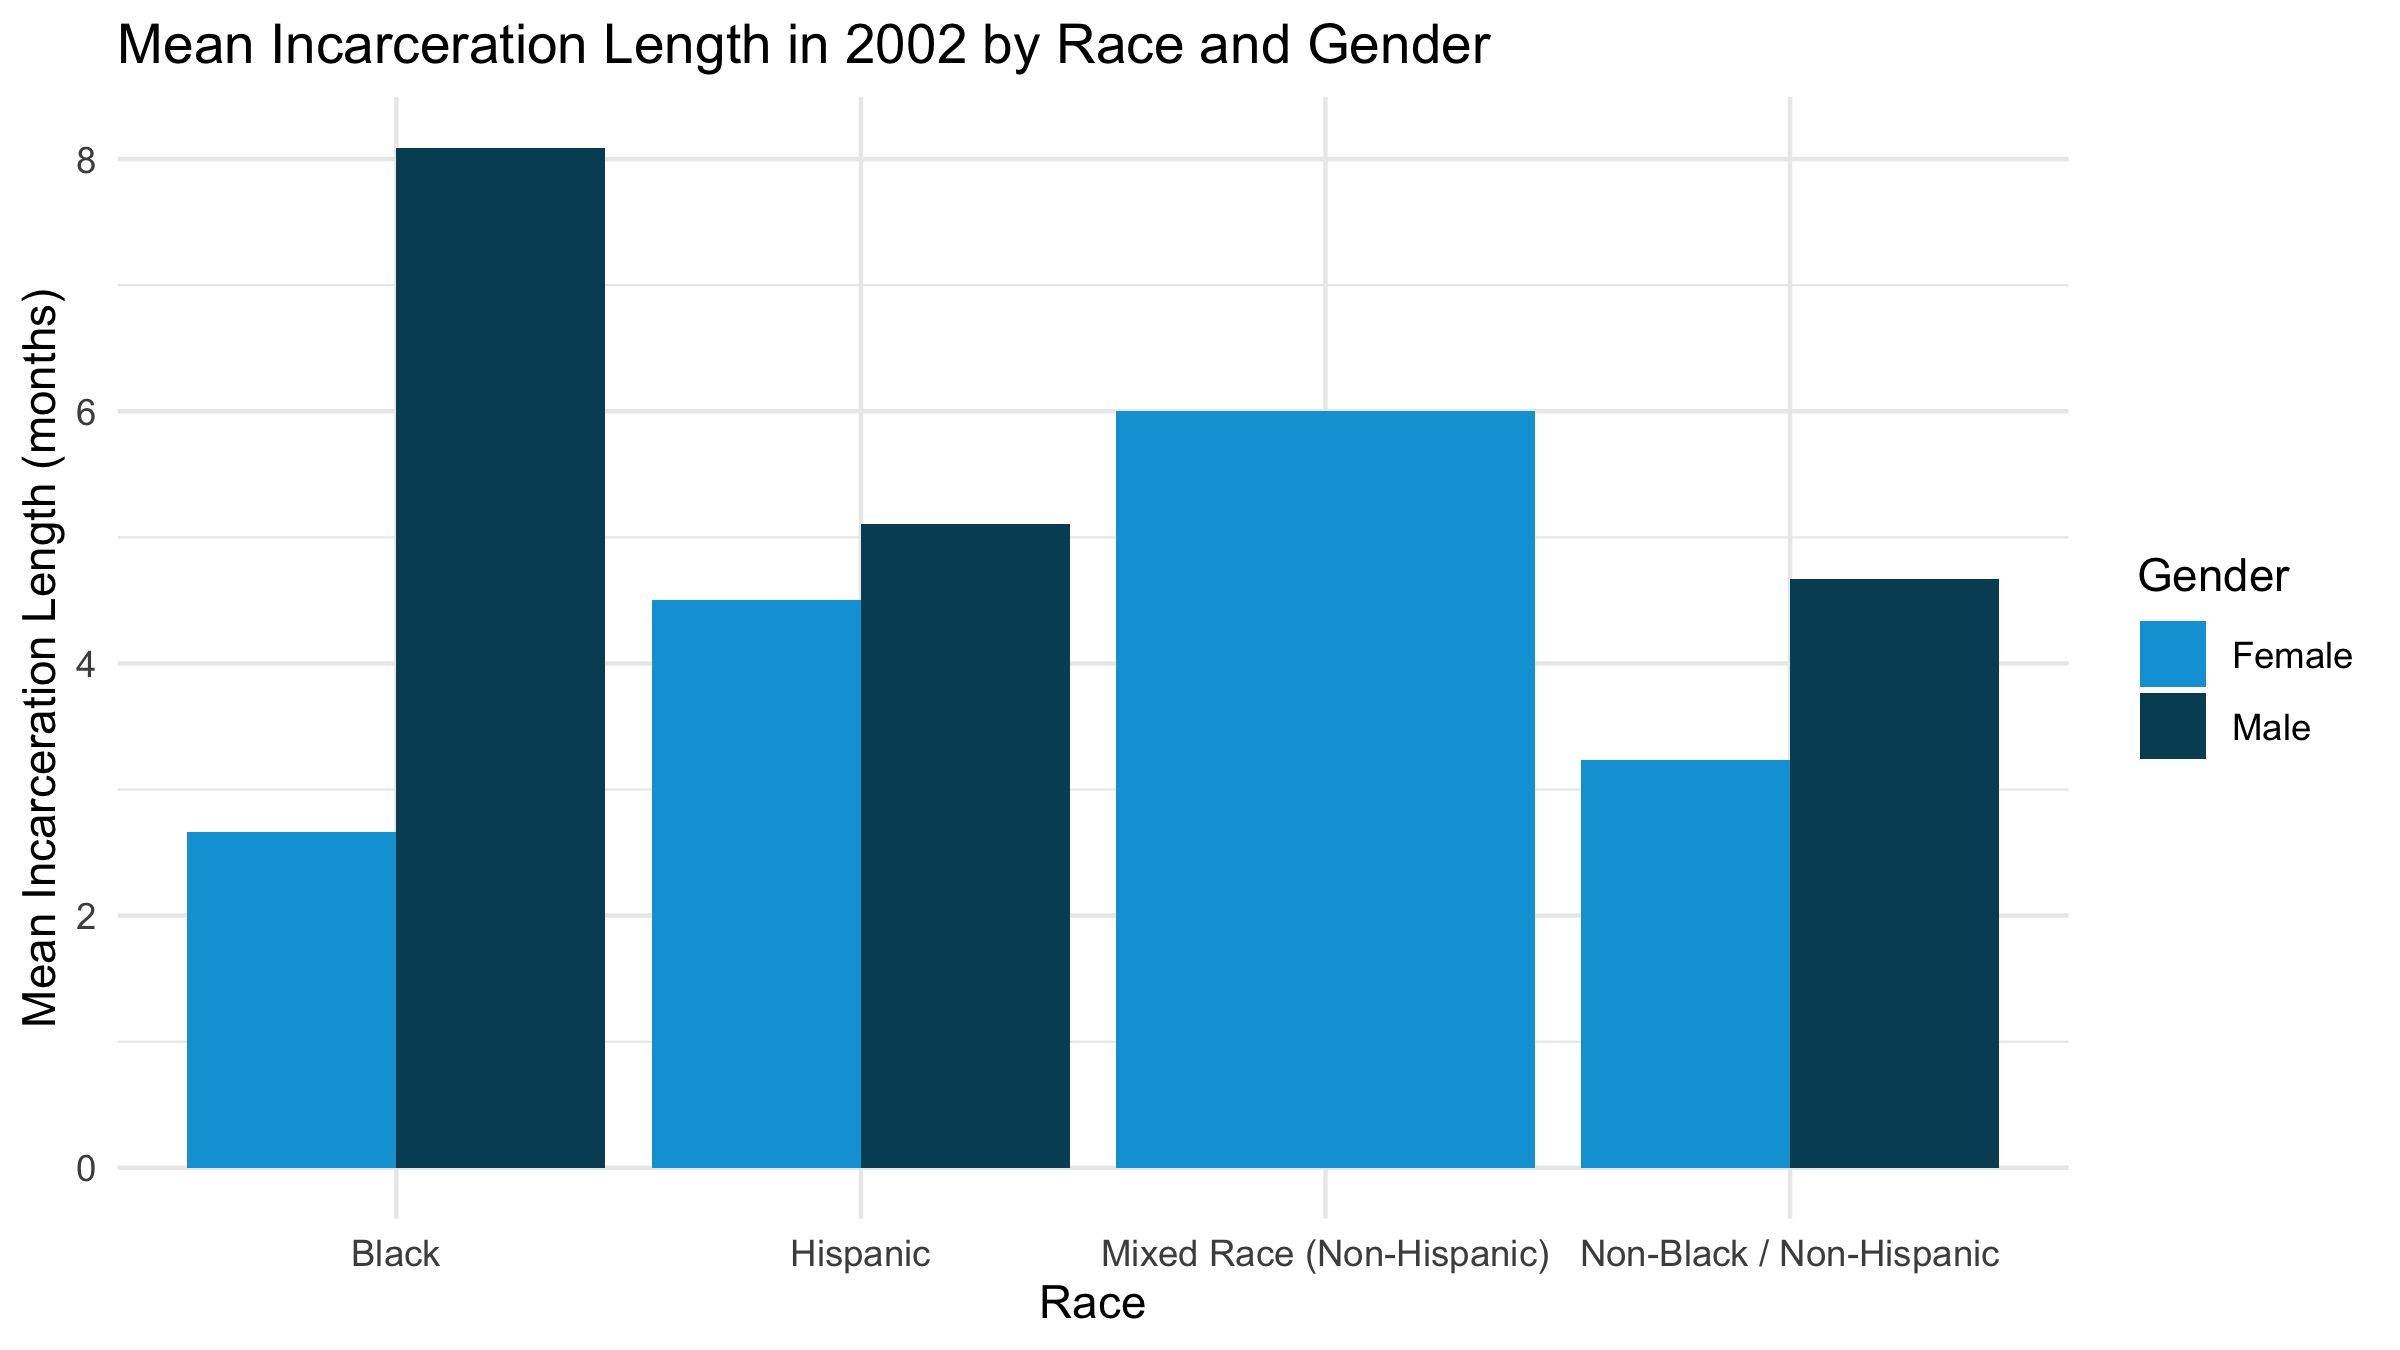
\includegraphics[width=.85\textwidth]{incarc_length_by_racegender}
    \end{center}
    \caption{Mean Incarceration Length in 2002 by Race and Gender}
    \label{fig:graph}
\end{figure}



\begin{table}[H]

\caption{\label{tab:tab:summarystats}Mean incarceration length in 2002 by Race and Gender}
\centering
\begin{tabular}[t]{lrrrr}
\toprule
Gender & Black & Hispanic & Mixed Race Non Hispanic & Non Black Non Hispanic\\
\midrule
\cellcolor{gray!6}{Female} & \cellcolor{gray!6}{2.666667} & \cellcolor{gray!6}{4.500000} & \cellcolor{gray!6}{6} & \cellcolor{gray!6}{3.230769}\\
Male & 8.090909 & 5.103448 & NA & 4.666667\\
\bottomrule
\end{tabular}
\end{table}



% Table created by stargazer v.5.2.2 by Marek Hlavac, Harvard University. E-mail: hlavac at fas.harvard.edu
% Date and time: Wed, Feb 16, 2022 - 15:39:03
\begin{table}[!htbp] \centering 
  \caption{Regression Output. Omitted category is Black Females.} 
  \label{tab:regression} 
\begin{tabular}{@{\extracolsep{5pt}}lc} 
\\[-1.8ex]\hline 
\hline \\[-1.8ex] 
 & \multicolumn{1}{c}{\textit{Dependent variable:}} \\ 
\cline{2-2} 
\\[-1.8ex] & Incarceration length in 2002 \\ 
\hline \\[-1.8ex] 
 Hispanic & $-$2.306 \\ 
  &  \\ 
  & \\ 
 Mixed Race (Non-Hispanic) & 0.857 \\ 
  &  \\ 
  & \\ 
 Non-Black / Non-Hispanic & $-$2.859 \\ 
  &  \\ 
  & \\ 
 Male & 2.610 \\ 
  &  \\ 
  & \\ 
 Constant & 5.143 \\ 
  &  \\ 
  & \\ 
\hline \\[-1.8ex] 
Observations & 178 \\ 
R$^{2}$ & 0.161 \\ 
Adjusted R$^{2}$ & 0.142 \\ 
Residual Std. Error & 3.946 (df = 173) \\ 
F Statistic & 8.302$^{***}$ (df = 4; 173) \\ 
\hline 
\hline \\[-1.8ex] 
\textit{Note:}  & \multicolumn{1}{r}{$^{*}$p$<$0.1; $^{**}$p$<$0.05; $^{***}$p$<$0.01} \\ 
\end{tabular} 
\end{table} 


\end{document}
